\section{Cointegration Testing Between Global Oil and LNG Spot Prices}

In addition to assessing the impacts of the Russian-war in Ukraine on the volatility of both oil and LNG
prices, we assessed the long run relationship between oil and LNG prices in order to deduce whether a
shock primarily associated with one commodity (i.e., sanctions on oil production and export) may
significantly impact the price of another commodity (LNG). In order to assess this, we ran the Johansen trace
test for cointegrated relationships on weekly spot prices for Brent crude (oil) and the Henry Hub spot price
for LNG.
\medskip

Previous research into the relationship between oil and LNG has supported the existence of an “unstable”
cointegrated relationship in the United States, wherein the short-run relationship between the two
commodities is highly influenced by supply shocks such as tropical storms and seasonal factors \cite{matt1}.
This led us to examine the possible impacts a sudden demand shock (such as sanctions)
may have upon the relationship between these commodities.
\medskip

The Johansen trace test for cointegration is used to test for the existence and magnitude of cointegrating
relationships between two or more time-series. In order to run the Johansen trace test, the data sets used
must be non-stationary. As such, we ran augmented Dickey-Fuller (ADF) tests on both time series with and
without a trend. Lags were chosen using the Akaike Information Criteria (AIC) and were all equal to 1. 
\medskip

As the data in table \ref{Tab:ADF_LNG} exhibits non-stationarity without a trend, we then run the Johansen test for these time series both with a linear trend in cointegration, and without. The results are outlined in Table \ref{Tab:Johansen}.

\begin{table}[H]
\centering
% \setlength{\tabcolsep}{5pt} % Default value: 6pt
% \renewcommand{\arraystretch}{1.5} % Default value: 1
\caption{Johansen Test Results}
\begin{tabular}{c|ccc}
            & Null & Critical Value & Lag Order\\\hline\hline
No Trend & $r = 1$ & 8.34* & 2\\\hline
Linear Trend & $r = 0$ & 8.66 & 2
\end{tabular}\label{Tab:Johansen}
\\
* Significant at the 5\% level\\
** Significant at the 1\% level
\end{table}

The results from the Johansen test show that, in a model without a linear trend, there is evidence for a
cointegrating relationship between oil and LNG spot prices, however, in a model with a linear trend, there is
not. Prior research has found evidence that, at least for oil prices, there does appear to be a linear
deterministic trend \cite{matt2}. Taking this into account, we focus on the cointegrating
relationship with a linear deterministic trend, finding that there is no clear evidence of a cointegrating
relationship between these time series. For the purpose of illustration, using the coefficients retrieved from
the Johansen test with a linear trend we produce the following, clearly non-stationary plot:

\begin{figure}[H]
    \centering
    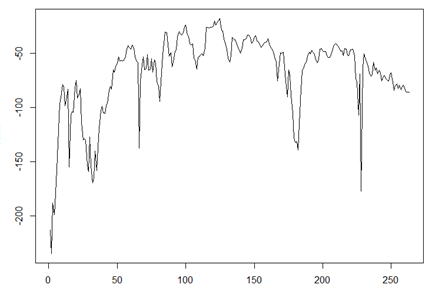
\includegraphics[width=0.6\textwidth]{Figures/Cointegration/non-stationary-plot.png}
    \caption{Non-Stationary Plot}
    \label{fig:Results_table}
\end{figure}

Running an ADF test on this model produces a test statistic that is not significant at the 5\% level ($p =
0.0972$), confirming that the relationship produced between the time series is indeed non-stationary.
Thus, we conclude that the impact of sanctions on one commodity is unlikely to significantly impact the
price of the other due to the existence of a cointegrating relationship. However it is possible that sanctions of one of
the commodities may affect the prices of the other through another channel.

